% vim:autoindent:set textwidth=78:

\section{Diseñador de mapas}\label{label_mapcomposer}

El diseñador de mapas es una función que proporciona capacidades limitadas de trazado e impresión. El diseñador le permite añadir elementos tales como la vista del mapa de QGIS, leyenda, barra de escala, imágenes y texto. Puede modificar el tamaño y la posición de cada elemento y ajustar las propiedades para crear su composición. El resultado se puede imprimir, exportar como imagen o exportarse a SVG.

Para acceder al diseñador de mapas, haga clic en el botón \textit{Imprimir} de la barra de herramientas o seleccione \textit{Imprimir} del menú \textit{Archivo}.

\subsection{Usar el diseñador de mapas}\label{label_usemapcomposer} 

Para usar el diseñador de mapas, primero añada las capas que quiera imprimir a QGIS. Debería representar y simbolizar las capas a su gusto antes de diseñar el mapa. 

\begin{figure}[ht]
   \begin{center}
   \caption{Diseñador de mapas}\label{fig:map_composer_blank}\smallskip
   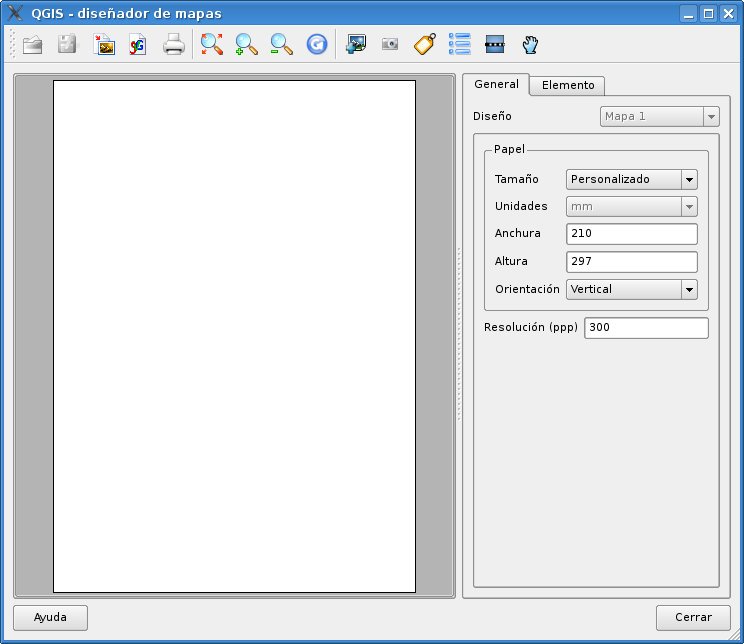
\includegraphics[clip=true, width=\textwidth]{map_composer_blank08}
\end{center}  
\end{figure}

Abrir el diseñador de mapas le proporciona un lienzo en blanco al que puede añadir la vista del mapa actual, leyenda, barra de escala y texto. La figura
\ref{fig:map_composer_blank} muestra la vista inicial del diseñador de mapas antes de que se añada ningún elemento.

El diseñador de mapas tiene dos pestañas: \textit{General} y \textit{Elemento}. La pestaña
\textit{General} permite establecer el tamaño del papel, la orientación y la resolución del mapa. La pestaña \textit{Elemento} muestra las propiedades del elemento seleccionado actualmente en el mapa. Seleccionando un elemento en el mapa (ej. leyenda, barra de escala, texto, etc.) y haciendo clic en la pestaña \textit{Elemento}, puede personalizar la configuración.

Puede añadir múltiples elementos al diseñador. Esto permite tener más de una vista de mapa y leyenda en el diseñador. Cada elemento tiene sus propias propiedades y en el caso del mapa, su propia extensión.

\subsubsection{Añadir un mapa al diseñador}

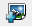
\includegraphics[width=0.7cm]{composer_add_map08} Para añadir la vista del mapa de QGIS al diseñador de mapas, haga clic en el botón \textit{Añadir mapa nuevo} en la barra de herramientasr. Arrastre un rectángule en el lienzo del diseñador para añadir el mapa. Puede redimensionar el mapa más tarde haciendo clic en el botón \textit{Seleccionar/Mover elemento}, haciendo clic en el mapa y arrastrando una de las asas de las esquinas del mapa. Con el mapa seleccionado, también puede redimensionarlo especificando la anchura y la altura en la pestaña de propiedades del elemento.

El mapa está enlazado con la vista del mapa de QGIS. Si cambia la vista en el lienzo del mapa haciendo zum o desplando, puede actualizar la vista del diseñador de mapas haciendo clic en el botón \textit{Actualizar vista}. También puede cambiar la vista del diseñador especificando una escala de mapa. Para establecer la vista a una escala determinada:

\begin{enumerate}
\item Seleccione \textit{Escala (calcular extensión)} del cuadro de lista \textit{Establecer}.
\item Introduzca el denominador de la escala en el cuadro de escala.
\item Pulse Intro.
\end{enumerate} 

\subsubsection{Añadir otros elementos al diseñador} 
 

\includegraphics[width=0.7cm]{composer_open_template} Se pueden usar plantillas existentes de QGIS para cargar y adaptar fácilmente disposiciones de mapa. Para abrir una plantilla existente, haga clic en el botón \textit{Abrir plantilla}. Seleccione una plantilla y personalice su apariencia. 

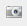
\includegraphics[width=0.7cm]{composer_add_image} Para añadir un logotipo, flecha de Norte o cualquier clase de imagen al diseñador, haga clic en el botón \textit{Añadir imagen}. La imagen se situará en el lienzo del diseñador y la podrá mover donde desee. 

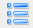
\includegraphics[width=0.7cm]{composer_add_legend08} Se puede añadir una leyenda al lienzo del diseñador y personalizarla para mostrar sólo las capas deseadas. Para añadir una leyenda, haga clic en el botón \textit{Añadir nueva leyenda vectorizada}. La leyenda se situará en el lienzo del diseñador y la podrá mover donde desee. Haga clic en la pestaña \textit{Elemento} para personalizar el aspecto de la leyenda, incluyendo qué capas se muestran.


\includegraphics[width=0.7cm]{composer_add_scalebar08} Para añadir una barra de escala al diseñador, haga clic en el botón \textit{Añadir nueva barra de escala}. Use
la pestaña \textit{Elemento} para personalizar el tamaño y número de segmentos y las unidades, tamaño y fuente de la escala.

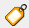
\includegraphics[width=0.7cm]{composer_add_label} Puede añadir etiquetas de texto al diseñador haciendo clic en el botón \textit{Añadir etiqueta nueva}. Use la pestaña \textit{Elemento} mientras el texto está seleccionado para personalizar la configuración o cambiar el texto predeterminado.

La figura \ref{fig:map_composer_complete} muestra el diseñador de mapas después de añadir cada tipo de elemento del mapa.
\begin{figure}[h]
   \begin{center}
   \caption{Diseñador de mapas con la vista del mapa, leyenda, barra de escala y texto añadidos}\label{fig:map_composer_complete}\smallskip
   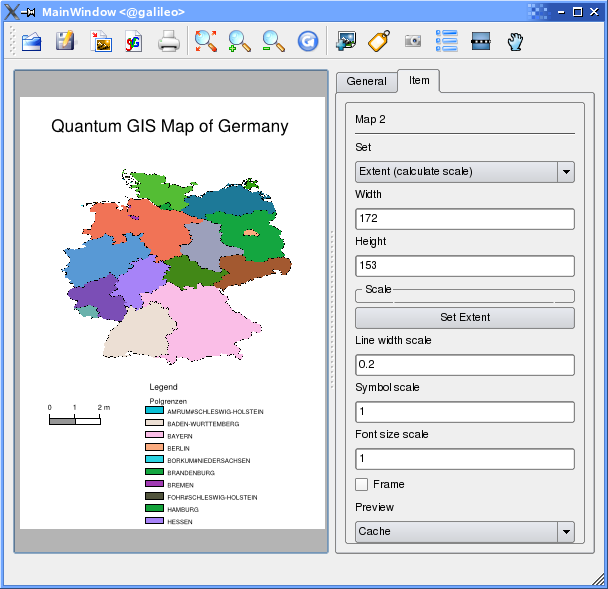
\includegraphics[clip=true, width=\textwidth]{map_composer08}
\end{center}  
\end{figure}

\subsubsection{Otras funciones}

El diseñador de mapas tiene herramientas de navegación para acercar y alejar el zum. Para acercar el zum, haga clic en la herramienta \textit{Acercar zum}. El lienzo del diseñador de mapas se ampliará en un factor de 2. Use las barras de desplazamiento para ajustar la vista al área de interés. Alejar con zum funciona de forma similar.

Si encuentra la vista en un estado inconsistente, puede usar el botón \textit{Actualizar vista} para volver a dibujar el lienzo del diseñador.

\subsubsection{Crear la salida}

El diseñador de mapas le permite imprimir el mapa en una impresora, exportarlo a PNG o a SVG. Cada una de estas funciones está disponible desde la barra de herramientas del diseñador.


\includegraphics[width=0.7cm]{composer_save_template} Para guardar el lienzo del diseñador como plantilla, haga clic en el botón \textit{Guardar plantilla como}. Busque el directorio que desee y guarde la plantilla para usarla de nuevo para otro mapa.

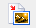
\includegraphics[width=0.7cm]{composer_export_image} Es posible exportar el resultado como una imagen haciendo clic en el botón \textit{Exportar como imagen}. 

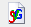
\includegraphics[width=0.7cm]{composer_export_svg} Para exportar el lienzo del diseñador como un SVG (Gráfico vectorial escalable), haga clic en el botón \textit{Exportar como SVG}. 
\textbf{Nota:} Actualmente la salida SVG es muy básica. Esto no es un problema de QGIS, sino de la biblioteca subyacente Qt. Esto se solucionará en versiones futuras.
 